\fancyhead{}
\fancyfoot{}
\cfoot{\thepage}


\lhead{Herramientas tecnologicas}

\chapter{Herramientas tecnologicas}
\section{Herramientas tecnologicas}
En el proceso de selección de herramientas para el desarrollo web, se consideraron los lenguajes de programación más reconocidos y utilizados en la industria. \\
Entre ellos se destacan: \\
Python: Conocido por su sintaxis sencilla y legibilidad, Python facilita el desarrollo rápido y eficiente de aplicaciones web. Su versatilidad y amplia gama de bibliotecas lo convierten en una opción atractiva para proyectos que requieren procesamiento de datos, inteligencia artificial o aprendizaje automático \cite{K}. \\
Java: Reconocido por su robustez y escalabilidad, Java es ampliamente utilizado en aplicaciones empresariales de gran envergadura. Su capacidad para manejar múltiples hilos de ejecución y su fuerte tipado lo hacen ideal para proyectos que demandan alto rendimiento y seguridad \cite{B}. \\
PHP: Diseñado específicamente para el desarrollo web, PHP es una opción popular para la creación de sitios dinámicos. Su integración sencilla con bases de datos y su amplia comunidad de desarrolladores proporcionan numerosos recursos y frameworks que agilizan el proceso de desarrollo. \cite{15} \\
\subsection{Proceso para elegir}
Para elegir la herramienta más adecuada para el desarrollo de mi sistema experto, comencé por considerar tres lenguajes de programación ampliamente utilizados: Python, PHP y Java. Mi enfoque inicial fue estudiar las características y ventajas de cada uno, lo que me permitió obtener una comprensión más clara de sus capacidades. \\
Primero, investigué en foros especializados para leer las reseñas y opiniones de otros desarrolladores sobre cada lenguaje. Esto me permitió conocer las experiencias de usuarios que ya habían trabajado con estas tecnologías y obtener información práctica sobre sus beneficios y limitaciones. \\
A continuación, utilicé Google Trends \cite{go} para analizar la popularidad de cada lenguaje en el tiempo y observar cuáles eran más buscados y utilizados en el contexto actual. Este análisis me ayudó a comprender las tendencias del mercado y cómo se posicionaban los lenguajes en el ámbito profesional. \\
Después, consulté el índice TIOBE \cite{to}, un sitio de referencia que mide la popularidad de los lenguajes de programación, para evaluar el posicionamiento global de Python, PHP y Java. Esto me brindó una visión más amplia sobre cuál de estos lenguajes era más robusto y preferido por la comunidad de desarrolladores. \\
Con toda esta información recopilada, organicé los datos en una tabla comparativa que incluía aspectos clave como la facilidad de aprendizaje, la velocidad de desarrollo, la disponibilidad de recursos y documentación, y la compatibilidad con el tipo de sistema que quería desarrollar. Finalmente, teniendo en cuenta tanto mis capacidades como novato como la fecha de entrega del trabajo, asigné puntuaciones a cada herramienta y, con base en los resultados, decidí optar por Python, debido a su curva de aprendizaje amigable y su extensa comunidad de apoyo. \\

\subsection{Descripción de las herramientas}
¿Qué es Python? \\
En términos técnicos, Python es un lenguaje de programación de alto nivel, orientado a objetos, con una semántica dinámica integrada, principalmente para el desarrollo web y de aplicaciones informáticas. \\
¿Qué es java? \\
Java es una plataforma informática de lenguaje de programación creada por Sun Microsystems en 1995. Ha evolucionado desde sus humildes comienzos hasta impulsar una gran parte del mundo digital actual, ya que es una plataforma fiable en la que se crean muchos servicios y aplicaciones. \\
¿Qué es php? \\
Php es un lenguaje de código abierto muy popular especialmente adecuado para el desarrollo web y que puede ser incrustado en HTM \\


\subsection{Grafico de las herramientas mas buscadas en google}
\begin{figure}[H]
    \begin{center}
    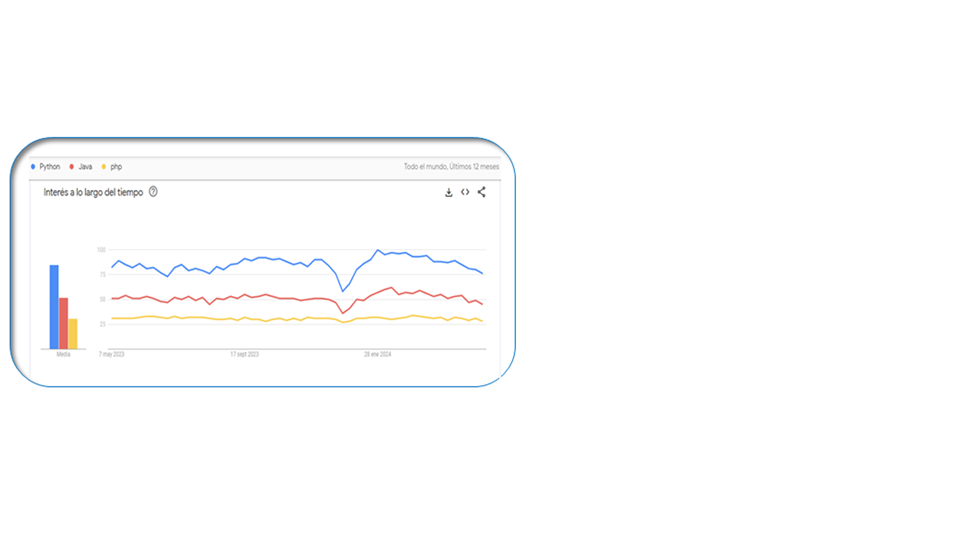
\includegraphics[scale = 1.1]{./images/Google trends.png}
    \caption{Google trends.}
    \label{fig:huella}
    \end{center}
    \end{figure}
En esta tabla, la organización Tiobe nos presenta los lenguajes de programación más buscados en varias plataformas de búsqueda [16]. \\

\subsection{Top 10 de las herramientas mas buscadas en el mundo}

\begin{figure}[H]
    \begin{center}
    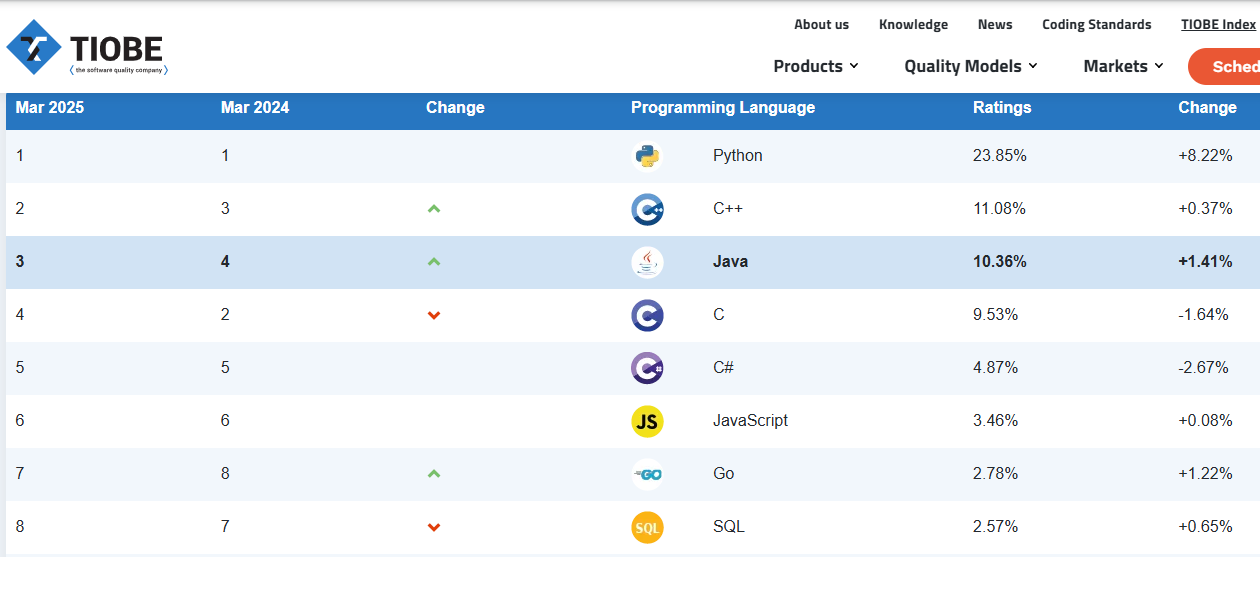
\includegraphics[scale = .4]{./images/tiobe.1.png}
    \caption{Organizacion tiobe.}
    \label{fig:huella}
    \end{center}
    \end{figure}

\subsection{Gráfico de los tres primeros lenguajes en el mundo.} 

Claramente Python está llevando el primer lugar en el último año. \\

\begin{figure}[H]
    \begin{center}
    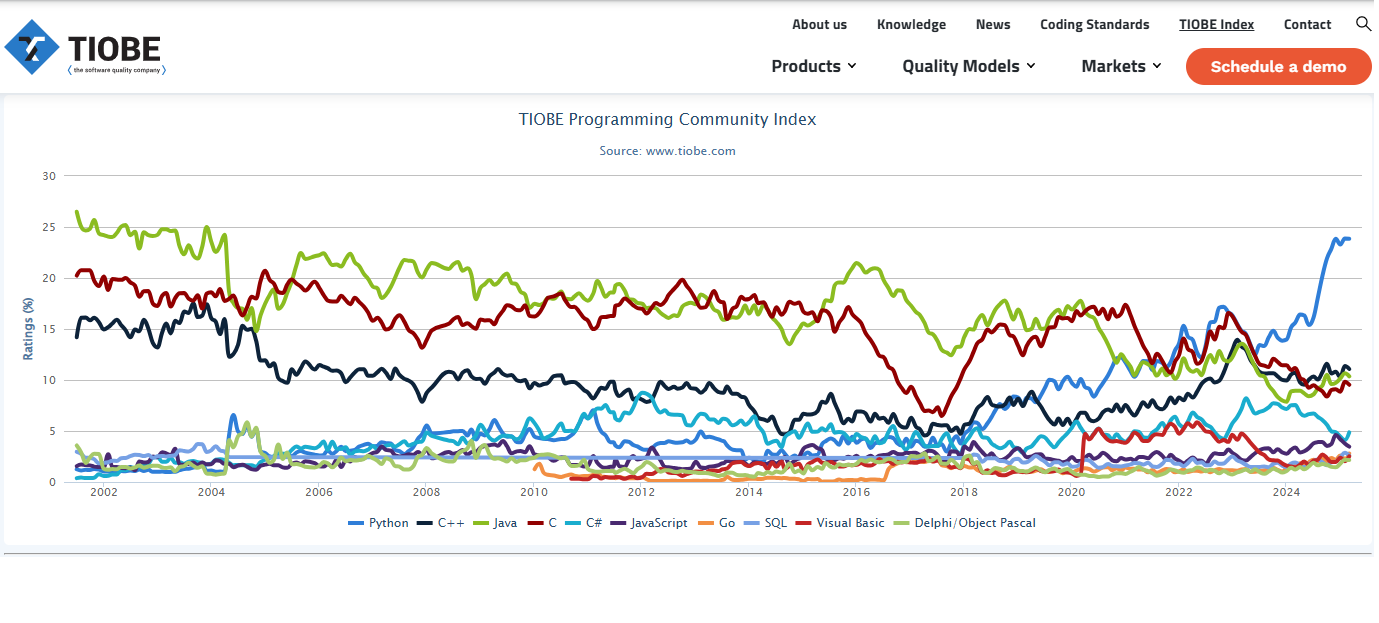
\includegraphics[scale = .4]{./images/tiobe.png}
    \caption{Organizacion tiobe.}
    \label{fig:huella}
    \end{center}
    \end{figure}
\subsection{Características de las herramientas.}

Las características de Python son los siguientes: \\
Python es un lenguaje interpretado, lo que significa que ejecuta directamente el código línea por línea, si existen errores en el código del programa, su ejecución se detiene, así, los programadores pueden encontrar errores en el código con rapidez.
Es un lenguaje fácil de utilizar porque utiliza palabras similares a las del inglés, a diferencia de otros lenguajes de programación, Python no utiliza llaves, en su lugar utiliza sangría. 
Es un lenguaje tipeado dinámicamente, los programadores no tienen que anunciar tipos de variables cuando escriben código porque Python los determina en el tiempo de ejecución. Debido a esto, es posible escribir programas de Python con mayor rapidez.
Es un lenguaje de alto nivel, Python es más cercano a los idiomas humanos que otros lenguajes de programación. Por lo tanto, los programadores no deben preocuparse de sus funcionalidades subyacentes, como la arquitectura y la administración de la memoria.
Es un lenguaje orientado a los objetos, Python considera todo como un objeto, pero también admite otros tipos de programación, como la programación estructurada y la funcional \cite{Bl}. \\

Las características de Java son las siguientes: \\
Es un lenguaje estable, al ser un lenguaje de programación sumamente estable, Java es elegido por las grandes empresas de todo el mundo que desean una tecnología confiable para sus proyectos. Debido a su confiabilidad y credibilidad, las compañías líderes lo incorporan para garantizar que la experiencia de los clientes sea la esperada.
Como lenguaje altamente escalable, Java ofrece capacidades de gestión de tráfico sin rival en ningún otro lenguaje. Esta escalabilidad lo ha convertido en una tecnología fiable para el desarrollo empresarial. Brinda un conjunto de funcionalidades que permite desarrollar aplicaciones web dinámicas e interactivas.
Cuenta con funciones de seguridad integradas que les facilitan a las empresas la protección adecuada de sus datos. Podemos destacar, entre otras características, la autenticación avanzada, los controles de acceso, la encriptación y las inyecciones de SQL. Asimismo, Java tiene funciones para integrar políticas de seguridad, firmas digitales y cifrados.
En Java, existen cientos de bibliotecas que admiten el desarrollo de aplicaciones empresariales. Estas bibliotecas permiten agregar características y funcionalidades de varios tipos, entre las que se incluyen: Google Guava, iText, Protocol Buffers y XStream. Asimismo, hay un amplio conjunto de APIs y herramientas de desarrollo que le facilitan a los desarrolladores añadir funciones que, de otra forma, no serían posibles.
Java funciona muy bien con el ecosistema de Android para crear aplicaciones móviles. Por eso, cada vez son más las empresas que eligen este lenguaje de programación para el desarrollo de aplicaciones Android nativas.
Es la facilidad con la que un software puede ejecutarse sobre diferentes plataformas informáticas, dependiendo lo menos posible de su entorno de ejecución y sin implementar las particularidades de una máquina o sistema concreto. Esto lo logra compilando a código que se ejecuta en una «máquina virtual» de Java. Por ello, puede ejecutarse tanto en entornos Windows como Linux \cite{Tec}. \\

Características de php: \\
Es un código abierto y gratuito. Es un lenguaje orientado a objetos, lo que hace el procesamiento de datos mucho más rápido. 
Permite la separación de códigos, es decir, es posible manipular datos mientras que otros se encuentran estáticos y también es un código limpio y estable. 
Cuenta con una comunidad amplia y activa donde es posible compartir conocimientos y encontrar información. Permite el desarrollo de páginas web complejas y dinámicas. 
Existe una amplia oferta laboral, pues hoy en día son cada vez más las compañías que buscan el desarrollo de sitios web particulares. 
Es un lenguaje que puede ejecutarse en cualquier servidor o sistema operativo siempre y cuando el equipo tenga la capacidad de ejecutar el código sin dificultades por lo tanto es un lenguaje versátil que permite un gran manejo de procesamiento de datos \cite{ph} \\

\subsection{Criterios de evaluación}
Multiplataforma: Se refiere a la capacidad de un lenguaje de programación o software para ejecutarse en múltiples sistemas operativos (Windows, macOS, Linux, etc.) sin necesidad de modificaciones significativas. \\
Software libre: Hace referencia a software que se distribuye con una licencia que permite a los usuarios usarlo, modificarlo y distribuirlo libremente.  \\
Software basado en red: Esto se refiere a aplicaciones o lenguajes de programación diseñados para funcionar o ser ejecutados en un entorno de red, como aplicaciones web o servicios en la nube. \\
Integración de datos: Se refiere a la capacidad del lenguaje o software para conectarse, interactuar y trabajar con diferentes fuentes de datos, como bases de datos SQL, NoSQL, servicios web, etc. \\
Tiempo de implementación: Se refiere al tiempo que se tarda en desarrollar y poner en producción una aplicación o sistema utilizando un lenguaje de programación o software. Esto puede variar según la complejidad del proyecto, la experiencia del desarrollador y las herramientas disponibles. \\
Curva de aprendizaje: Hace referencia a la facilidad con la que los nuevos usuarios pueden aprender a utilizar un lenguaje de programación o software. 

Tablas de comparación \\
\begin{figure}[H]
    \begin{center}
    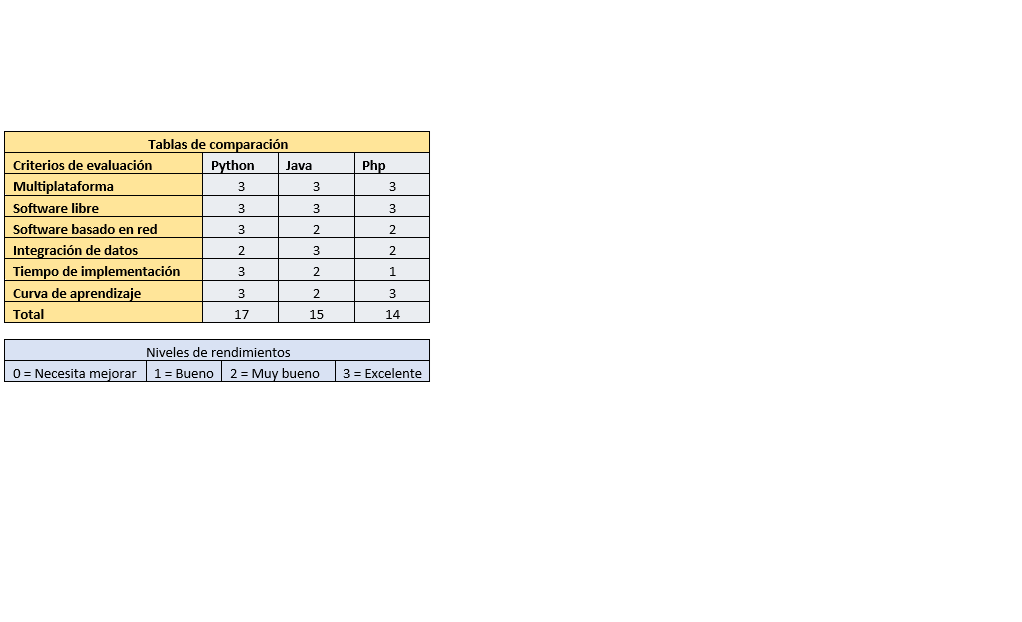
\includegraphics[scale = 1.1]{./images/Tablas de comparacion.png}
    \caption{Tabla de comparacion.}
    \label{fig:huella}
    \end{center}
    \end{figure}

\subsection{Tecnología seleccionada}
Tras analizar diversas opciones, encontramos múltiples herramientas capaces de llevar a cabo el desarrollo de la aplicación requerida. Sin embargo, la elección se basó en criterios clave como la compatibilidad multiplataforma, el corto tiempo de implementación y una curva de aprendizaje más accesible en comparación con otros lenguajes de programación evaluados. \\
En función de estos criterios, la tecnología seleccionada para el desarrollo es Python, debido a su versatilidad, facilidad de uso y amplia comunidad de soporte. \\
Otras tecnologías. \\
Además del lenguaje de programación, el sistema utilizará PostgreSQL como motor de base de datos. PostgreSQL es un sistema gestor de bases de datos relacional, libre y de código abierto, reconocido por su robustez y escalabilidad. Para la administración y gestión de la base de datos, se empleará pgAdmin, una herramienta gráfica que facilita la configuración, monitoreo y mantenimiento del sistema \cite{doc}. \\
